\documentclass[a4paper,12pt,openany]{book}
\usepackage[hidelinks]{hyperref}
\usepackage[nottoc]{tocbibind}
\usepackage[toc,page]{appendix}
\usepackage[utf8]{inputenc}
\usepackage{color}
\usepackage{datetime}
\usepackage{ragged2e}
\usepackage{graphicx}
\usepackage{listings, listings-rust}
\usepackage{multirow}
\usepackage{pgfplots}
\usepackage{quoting}
\usepackage{textcomp}
\usepackage{url}
\usepackage{xcolor}
\usepackage{xparse}

% \usepackage[style=numeric-comp]{biblatex}
% \addbibresource{bibliography.bib}

\graphicspath{ {./images/} }

\hypersetup{breaklinks=true}
\urlstyle{same}


\definecolor{codegreen}{rgb}{0,0.6,0}
\definecolor{codegray}{rgb}{0.5,0.5,0.5}
\definecolor{codepurple}{rgb}{0.58,0,0.82}
\definecolor{backcolour}{rgb}{0.95,0.95,0.92}
\definecolor{rustcolor}{rgb}{0.87, 0.64, 0.51}
\definecolor{ocamlcolor}{rgb}{0.23, 0.88, 0.20}
\definecolor{pythoncolor}{rgb}{0.20, 0.44, 0.64}

\lstdefinestyle{mystyle}{
    % backgroundcolor=\color{backcolour},
    commentstyle=\color{codegreen},
    keywordstyle=\color{magenta},
    numberstyle=\tiny\color{codegray},
    stringstyle=\color{codepurple},
    basicstyle=\footnotesize\ttfamily,
    breakatwhitespace=false,
    breaklines=true,
    captionpos=b,
    keepspaces=true,
    numbers=left,
    numbersep=5pt,
    showspaces=false,
    showstringspaces=false,
    showtabs=false,
    tabsize=2
}

\lstdefinestyle{customc}{
  breaklines=true,
  numbers=left,
  numbersep=5pt,
  numberstyle=\tiny\color{codegray},
  frame=L,
  language=C,
  showstringspaces=false,
  basicstyle=\footnotesize\ttfamily,
  keywordstyle=\bfseries\color{green!40!black},
  commentstyle=\itshape\color{purple!40!black},
  identifierstyle=\color{blue},
  stringstyle=\color{orange},
}

\lstset{style=mystyle}

\NewDocumentCommand{\codeword}{v}{%
\texttt{\textcolor{blue}{#1}}%
}

\newdateformat{monthyeardate}{%
  \monthname[\THEMONTH] \THEYEAR}

\begin{document}

\begin{titlepage}
\sloppy
\begin{center}
\normalsize{BABEȘ-BOLYAI UNIVERSITY CLUJ-NAPOCA}\\
\normalsize{FACULTY OF MATHEMATICS AND COMPUTER SCIENCE}\\
\normalsize{SPECIALIZATION COMPUTER SCIENCE}\\
\end{center}

\vspace{2cm}
\begin{center}
\huge \textbf{DIPLOMA THESIS}\\
\vspace{1cm}
\Huge \textbf{GCSF -- A VIRTUAL FILE SYSTEM BASED ON GOOGLE DRIVE}
\end{center}

\vspace{2cm}

\begin{flushleft}
\textbf{Supervisor} \\
\textbf{Lect. dr. Mircea Ioan-Gabriel}
\end{flushleft}


\begin{flushright}
\textbf{Author} \\
\textbf{Pușcaș Sergiu Dan}
\end{flushright}

\vspace{1.5 cm}
\begin{center}
\Large{2018}
\end{center}

\end{titlepage}

% \frontmatter

\clearpage % end title page
\begingroup
  \pagestyle{empty}
  \null
  \newpage
\endgroup

\tableofcontents

\chapter{Introduction}

The past decade has brought the rise of cloud storage services as an extension of traditional disk-based storage systems. There are many options to choose from, and multiple ways of interacting with them. Chapter \ref{state_of_the_art}  analyses some of the most popular choices. This thesis will focus on a particular service -- Google Drive.

Unfortunately, business requirements encourage companies to target the largest demographic possible, in order to provide the best experience for the average user. This puts advanced users at a disadvantage. Chapter \ref{proposed_approach} aims to provide a solution tailored specifically for them. This solution comes in the form of a new desktop application for Unix-like systems, named GCSF. GCSF is a virtual file system built on top of Google Drive, allowing users to mount their account locally and interact with it as they would with a traditional disk-based storage system.

Chapter \ref{performance_evaluation} explores existing alternatives and compares them against GCSF, focusing on two aspects -- performance and user experience.

Finally, Chapter \ref{conclusion} provides some directions for further development and improvement, and reflects on the progress made since the beginning of this project.

\chapter{State of the art}

Cloud storage services have been steadily increasing in popularity and reached mainstream status in the past decade. In essence, these services allow users to upload and store files on the internet without the need to own the physical storage medium. Files can be accesed from almost any devices with an internet connection, provided that the user follows the required authentication process.

Most cloud storage services provide free plans, which usually limit the total storage capacity. Their premium plans either follow the subscription business model or even go as far as to require a one-time purchase in exchange for a lifetime subscription.

As of \monthyeardate\today, some of the most popular\cite{google_plans_to_leverage} names ring a bell even to non-technical users:
\begin{itemize}
\item Microsoft OneDrive
\item Google Drive (800 million active users, \date{March 2017})
\item Apple iCloud Drive
\item Box
\item Dropbox
\end{itemize}

This is no coincidence. Many tech companies attempt to draw users into their own ecosystem, especially when it is a vast one. Consumers that already use several products owned by the same company tend to favor that company's other products over their direct competitors. There are multiple advantages in doing so. For one, familiarity is a key factor. A competitor's service may be more difficult to use by a consumer who is unfamiliar with it. On top of that, a single ecosystem provides greater cohesion between its elements. This translates into better integration between services, which improves the overall experience.

Two of the largest technology companies -- \mbox{Apple Inc.} and \mbox{Alphabet Inc.} -- are commonplace examples of this strategy. Users who sign up for a free Gmail account automatically receive an associated \mbox{15 GB} storage plan on Google Drive. Moreover, this storage is shared among three different services: Google Drive, Gmail and Google Photos. Similarly, Apple offers \mbox{5 GB} of free storage on iCloud:

\begin{quote}
iCloud is built into every Apple device. That means all your stuff — photos, files, notes, and more — is safe, up to date, and available wherever you are. And it works automatically, so all you have to do is keep doing what you love. Everyone gets \mbox{5 GB} of free iCloud storage to start, and it’s easy to add more at any time.
\end{quote}

It seems that offering free storage is similar in concept to planting a seed that will reap a greater harvest. Indeed, making a user familiar with your service will make him more likely choose your premium plan when deciding to upgrade, instead of your competitor's.

\section{User Interface}

File hosting services usually allow access via \mbox{HTTP}, with some of them also supporting \mbox{FTP}. As a consequence, the main way of interacting with them is via a web platform.

\begin{figure}[tbp]
\caption{Web interface of the Dropbox file hosting service}
\centering
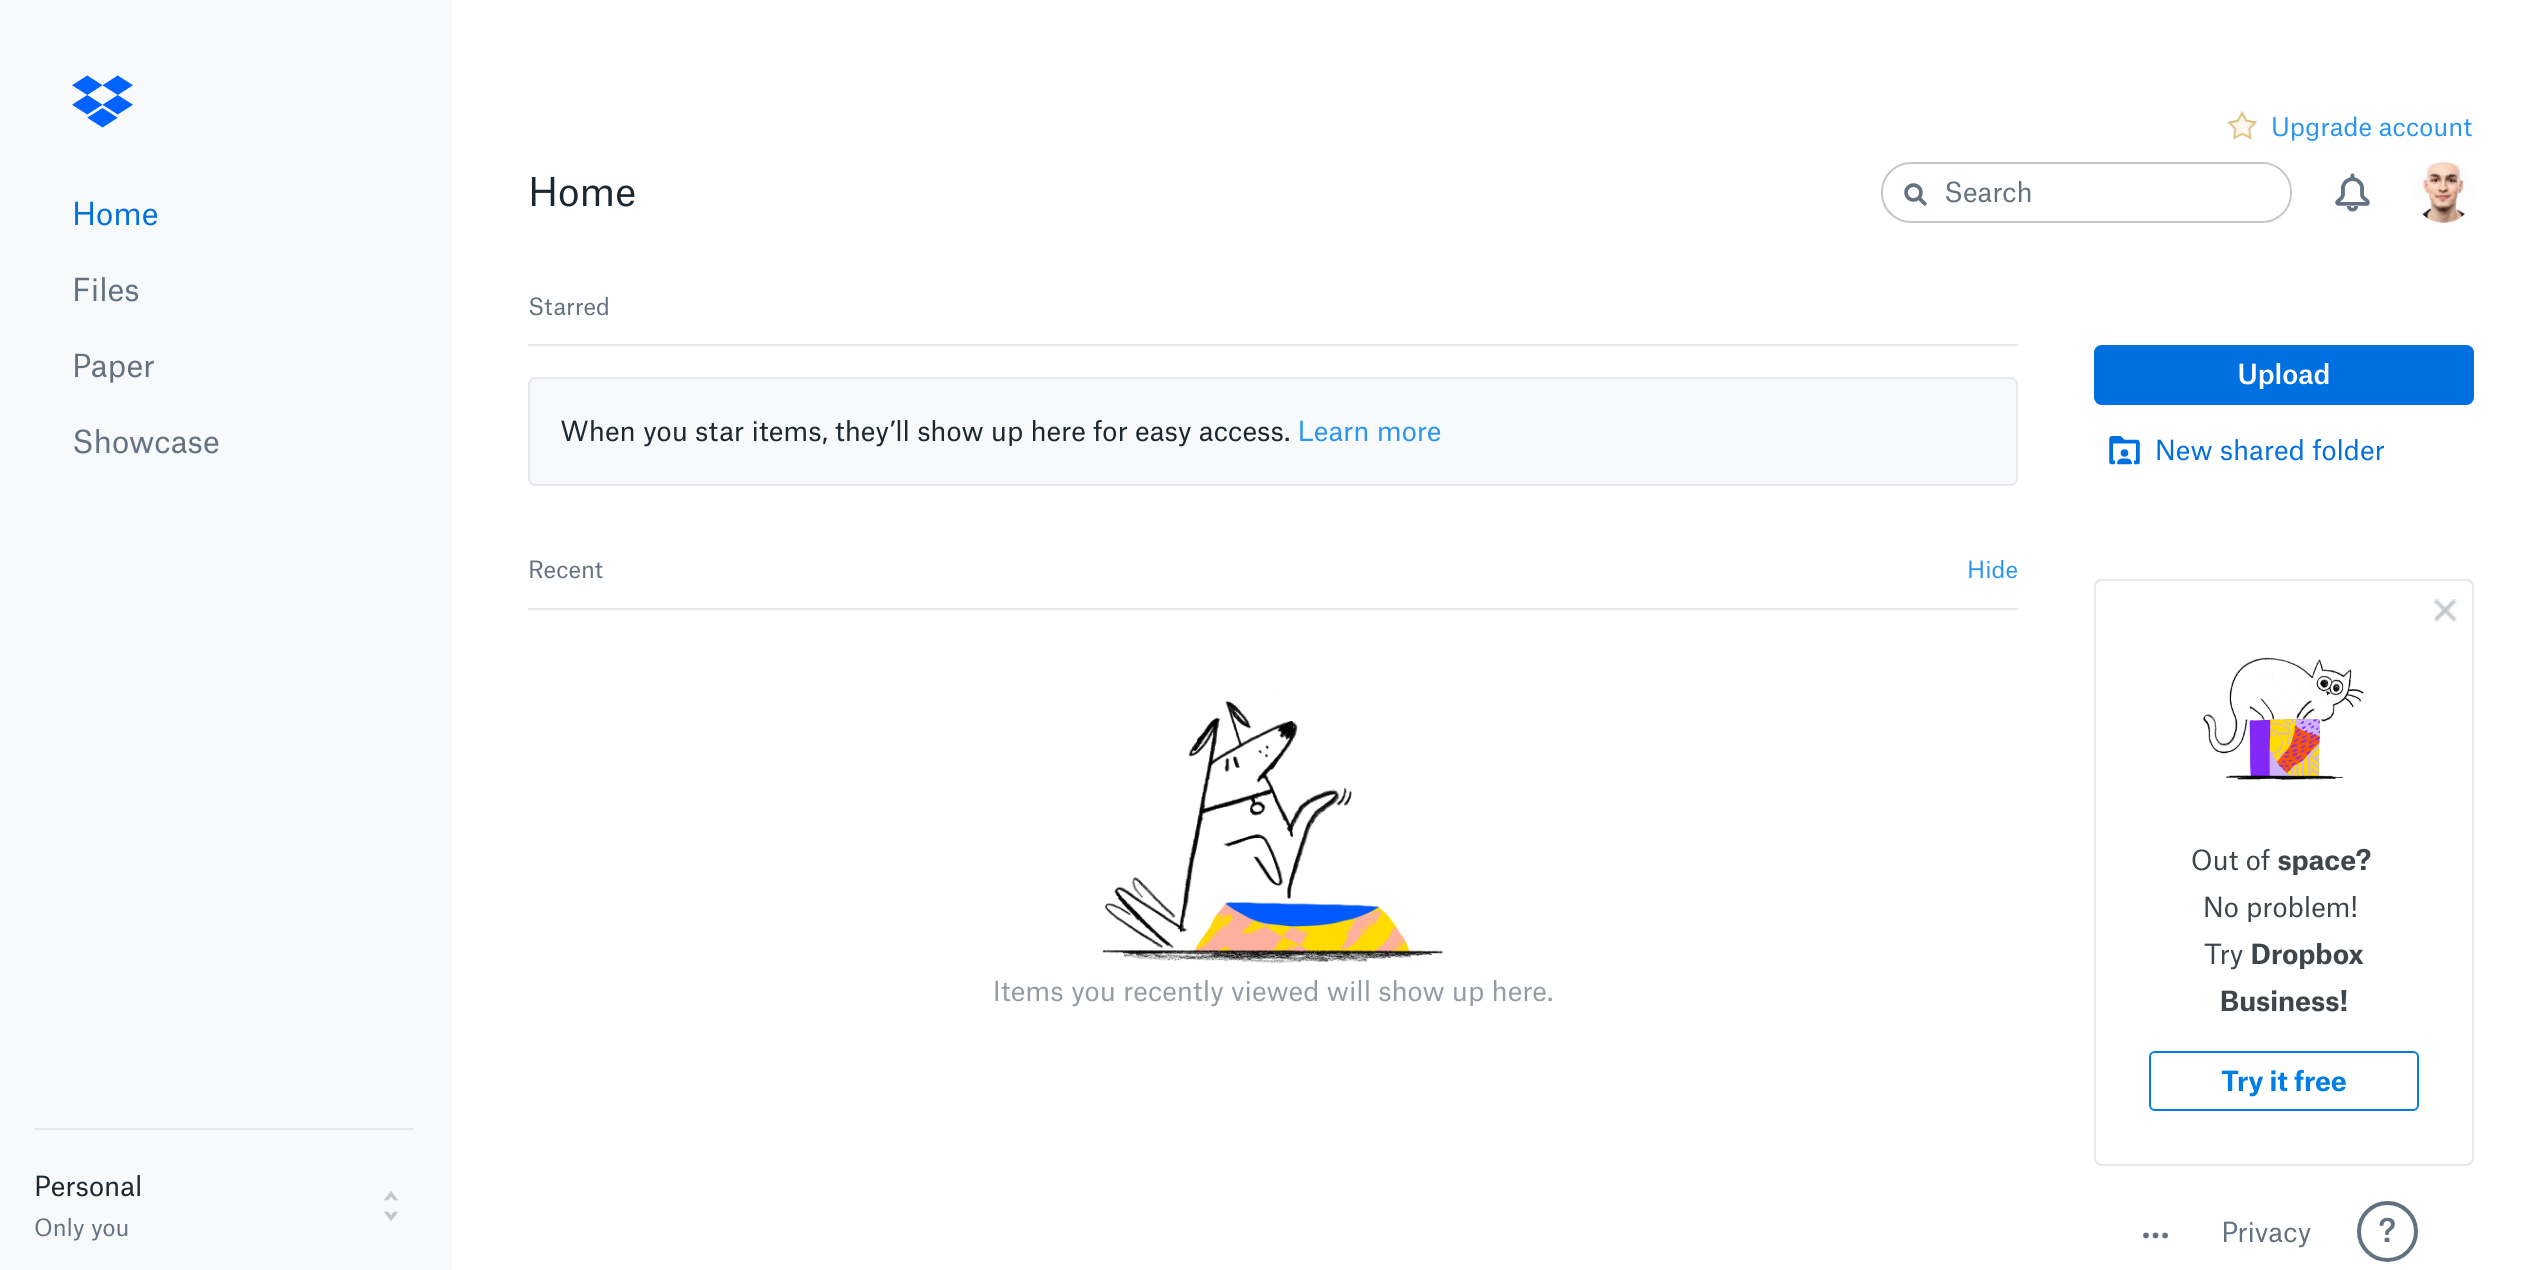
\includegraphics[width=\textwidth]{dropbox_homepage}
\end{figure}

These interfaces are updated regularly with new features and improved design. In \date{May 2018}, Google rolled out a new update\cite{google_drive_ui_updates} for Drive which is more in tune with its latest material design principles\cite{how_google_created_a_custom_material_theme}.

Mobile users also enjoy native applications for many file storage services. As of \monthyeardate\today, Google Drive for Android has been installed more than one billion times\footnote{\url{https://play.google.com/store/apps/details?id=com.google.android.apps.docs}}. Dropbox and OneDrive are close behind, with more than 500 million and 100 million installs, respectively\footnote{\url{https://play.google.com/store/apps/details?id=com.dropbox.android}}\footnote{\url{https://play.google.com/store/apps/details?id=com.microsoft.skydrive}}.

\section{File Sync}

Originally, file hosting services did not behave precisely as they do today. When Dropbox was initially founded in 2007, it did not rely on a web interface for its service. It did not even own the \emph{dropbox.com} domain.\footnote{\url{https://techcrunch.com/2009/10/13/dropbox-acquires-the-domain-everyone-thought-it-had-dropbox-com/}} Users had to download a desktop application from \emph{getdropbox.com} and run it locally, thus interacting with the service.

The application followed an approach that was mainly designed by Drew Houston, the company's CEO. The key element was a special folder added to the user's file system. This folder was then synced to all devices that were linked to the same Dropbox account. Any file placed in this folder would get sent to the cloud and become available to other devices.

The success of Dropbox convinced other companies to follow suit. Google Drive was introduced in \date{April 2012} for Windows, macOS and Android.\footnote{\url{https://googleblog.blogspot.ro/2012/04/introducing-google-drive-yes-really.html}} A few months later, an iOS application was launched as well.\footnote{\url{https://arstechnica.com/information-technology/2012/06/hands-on-with-the-google-drive-for-ios-app-mostly-read-only/}}.

In the same year, Google famously told users: ``We're working on Linux support--hang tight!''.\footnote{\url{https://www.pcworld.com/article/254488/google_drive_for_linux_is_on_the_way.html}} The announcement slowly went under the radar and the project was eventually cancelled. This gave birth to an infamous joke website\footnote{\url{https://abevoelker.github.io/how-long-since-google-said-a-google-drive-linux-client-is-coming/}} which counts how much time users have been waiting for the Linux client.

In \date{September 2017}, Google made another announcement regarding the desktop application. The official Drive app would be discontinued in \date{March 2018}, its place being taken by the new \emph{Backup and Sync} app.\footnote{\url{https://www.blog.google/products/photos/introducing-backup-and-sync-google-photos-and-google-drive/}}\footnote{\url{https://www.pcworld.com/article/3223136/data-center-cloud/google-drive-is-being-replaced-by-backup-and-sync-what-to-expect.html}}

It is easy to notice then that Linux users have been at a disadvantage ever since Drive was first launched. They essentially had three options:
\begin{itemize}
\item switch to a different file hosting service or operating system,
\item use the web platform, or
\item use unofficial third-party clients, which were usually bugged and lacked complete functionality.
\end{itemize}

\section{Main advantages}

\subsection{Cloud Storage}

For many consumers, file hosting services are used on a daily basis. Compared to traditional disk-based storage systems, cloud-based services provide several advantages. The most palpable one is data redundancy and backup. Users no longer risk the chance of losing their data due to a lost or stolen device or because of a hardware failure. Files that are stored in the cloud provide an extra layer of safety. On top of this, file sharing becomes almost trivial. What used to require manual transfers between different storage mediums (e.g. floppy disks, flash drives or external hard drives) is now done almost entirely automatically. It is enough to place the desired files in the special folder on a computer and they will magically appear on all other linked devices.

Indeed, this is the inconvenience that gave birth to Dropbox. Drew Houston founded the company after repeatedly forgetting his USB flash drive while being a student at MIT.

Another advantage is cross-platform integration. Over a third of the world's population owns a smartphone, and this number is expected to grow in the coming years.\footnote{\url{https://thehub.smsglobal.com/smartphone-ownership-usage-and-penetration}}. Therefore, file hosting services narrow the gap between traditional desktop computers and mobile phones.

Finally, the freemium model adopted by many of the services mentioned previously translates into free extra storage for everyday users. Even the paid plans are a strong competitor for traditional storage systems. In \date{2018}, the cost per gigabyte of storage commonly reaches values as low as \mbox{\textdollar 0.05\slash GB}.\footnote{\url{https://www.backblaze.com/blog/hard-drive-cost-per-gigabyte/}}. With Google Drive's most popular paid plan, this value is approximately 4 times lower: \mbox{\textdollar 0.012\slash GB\slash month}.\footnote{\url{https://www.google.com/drive/pricing/}} Although this is a recurrent cost, it often makes sense financially to opt for cloud storage, especially with all the other provided benefits.

\subsection{File Sync}

File syncing is in itself an enticing feature. Having a special folder on an existing file system comes with no additional learning curve. Any computer-literate user can instantly make sense of such a service and use it without prior preparation.

\subsection{Service Integration}

As discussed above, file sharing services are seldom provided by themselves. The best example of this is Google, which aims to merge most of its services into a cohesive and consistent user experience. Special files created in Google Docs, Forms, Sheets or Slides use Drive as the storage medium and integrate with it seamlessly. Files can easily be shared with Gmail contacts. Mail attachments can be saved to Drive with a single click. This improves workflow of many consumers globally. Teams no longer have to pass text documents back and forth; all members can edit the same document at the same time.

\section{Main disadvantages}

\subsection{Security}

Although useful in many aspects, the rise of file hosting services are a cause for worry for many users. One of the main concern comes from the risk associated with storing sensitive information on someone else's servers, making it vulnerable to data breaches and leaks.

Dropbox is just one case of controversy. In \date{June 2011} an authentication problem allowed the access of multiple accounts for several hours \emph{without} passwords.\footnote{\url{https://techcrunch.com/2011/06/20/dropbox-security-bug-made-passwords-optional-for-four-hours/}} In \date{August 2016}, 68 million accounts have been compromised by hackers who stole email addresses and hashed passwords.\footnote{\url{https://arstechnica.com/information-technology/2016/08/dropbox-hackers-stole-email-addresses-hashed-passwords-68m-accounts/}}

\subsection{Availability}

Throughout the years, web services in general have proved that 100\% reliability is unachievable in practice. Google offers a 99.9\% uptime guarantee for G Suite customers of Google Drive. However, there have been multiple outages since the service's initial launch in 2012:

\begin{itemize}
  \item \date{March 2013}\footnote{\url{https://techcrunch.com/2013/03/18/google-drive-experiencing-intermittent-issues/}}
  \item \date{October 2014}\footnote{\url{https://thenextweb.com/google/2014/10/27/google-drive-docs-users-company-investigating/}}
  \item \date{January 2016}\footnote{\url{https://www.independent.co.uk/life-style/gadgets-and-tech/news/gmail-google-drive-down-many-google-services-hit-by-widespread-outage-a6834711.html}}. Google later apologized:
    \begin{quote}
      At Google we recognize that failures are statistically inevitable, and we strive to insulate our users from the effects of failures. As that did not happen in this instance, we apologize to everyone who was inconvenienced by this event. Our engineers are conducting a post-mortem investigation to determine how to make our services more resilient to unplanned network failures, and we will do our utmost to continue to make Google service outages notable for their rarity.
    \end{quote}
  \item \date{September 2017}\footnote{\url{https://thenextweb.com/google/2017/09/12/google-down-gmail-youtube-maps/}}
\end{itemize}

These outages carry an immense impact on users. When all Google services went out for 5 minutes in \date{August 2013}, the total internet traffic dropped by 40\%.\footnote{\url{https://www.cnet.com/news/google-goes-down-for-5-minutes-internet-traffic-drops-40/}} Even so, Google Drive's reliability still beats that of user-owned hardware. Consumers are more likely to lose data because of their own hard drives failing than Google's. Still, the perceived effect is the opposite. When you lose your data, you might be tempted to pass it off as a fact of life. When Google loses your data, there is outrage, and rightly so.

\subsection{Power user experience} \label{power_user_experience}

Although cloud hosting services usually provide a first-rate user experience, they do not cover every possible use case. This is especially true when discussing about power users. For the purpose of this argument, I will use the following definition of the term:

\fbox{\textit{(noun)} \textbf{power user}: a knowledgeable and sophisticated user of computers.}

This includes students, professional programmers, hobbyists and all other computer users with a large knowledge base who like to tinker with computers in interesting and unexpected ways.

This description matches the traditional stereotype of a computer hacker. The term is known in popular press as someone who breaks into computers. However, it has a different meaning among programmers. In this context, a hacker is usually someone who strikes to achieve mastery by their own merit, being driven by curiosity more often than not. It is not necessarily a computer term: a famous anecdote regarding Nobel laureate Richard Feynman describes his pastime of breaking into safes containing secret documents just for the fun of it\cite{feynman}.

Hackers often create wealth by writing open source software and publishing it for the entire world to use and modify freely\cite{hackers_and_painters}. Plenty of them come into contact with programming at an early age and follow formal education only as a secondary way of learning. Hackers are seldom happy with their systems and their knowledge. They always seek new and better ways of making computers do what they want. Living in the terminal usually becomes the preferred way of getting things done.

For many of them, it is hard to take slow typists seriously as programmers. This is not an indicator of arrogance -- typing speed does not reflect one's ability as a programmer, but it does show much time one has spent using a computer, actually writing programs.

Although Linux has a modest market share of only 2.16\% for desktop and laptop usage\footnote{\url{https://goo.gl/QPcwGZ}}, it is far more popular with developers and power users, 48.3\% of them having used a variation of it for development work in \date{2018}.\footnote{\url{https://insights.stackoverflow.com/survey/2018/#technology}}

It is therefore unfortunate that the very people who create software are the ones who benefit the least from it, at least in the case of cloud hosting services. Forcing a power user to use a browser in order to share files can easily be an impediment to their productivity. The command line simply does not pair well with browser-based web services. Imagine wanting to write a script that uploads some backup file to such a service and having to implement it in a way that integrates it into the browser. This sort of automation task is not unheard of among power users, yet the lack of native Linux support makes it way harder than it has to be.

\chapter{Proposed approach}

\section{Aim}

This project aims to improve the experience of using Google Drive specifically for power users. Regular users can benefit from it as well -- provided they follow some prerequisite steps in order to use the application.

If successful, it will drastically diminish the issues described in \ref{power_user_experience}.

\section{Summary}

In essence, Google Drive is nothing more than a remote storage system. All the operations that a user might want to execute on a local storage system (e.g. copying files, creating and organising directories, reading and writing data) have an equivalent operation on Google Drive.

Disk-based storage devices are organized by the operating system using a filesystem in order to keep track of all the data they contain. This happens behind the scences. Users can interact with the storage device using system calls. Some of the more popular ones are \codeword{read}, \codeword{write}, \codeword{close}, \codeword{wait}, \codeword{exec}, \codeword{fork}, \codeword{exit}, \codeword{kill}. Note that not all of these deal with file storage. Some of them are a proxy which expose different functionalities of the operating system.

An interesting concept comes to mind: why not model a Google Drive account in such a way that it behaves identically to a traditional filesystem? The only difference would be that instead of storing and reading data from a local disk, it would interact with Google's servers.

GCSF does exactly that. It is a virtual filesystem on top of Google Drive. It allows users to mount their Drive account locally and interact with it as with a regular disk partition. This is achieved using the FUSE (Filesystem in Userspace) interface\footnote{\url{https://github.com/libfuse/libfuse}}, as described in \ref{implementation}.

\section{Usage}

Before delving into implementation details, I present a brief overview of how GCSF works from the user perspective.

GCSF consists of a single binary. When executed with no arguments, it prints a help menu as seen in \ref{gcsf_help_menu}. Users can choose to mount the filesystem to a local directory. GCSF points to an authentication URL (\ref{gcsf_mount}) that must be accessed in order to obtain the right credentials for Google Drive (fig.~\ref{fig:drive_auth}). Upon completing the authentication process, GCSF mounts the filesystem and populates it with all files and directories contained in the \emph{My Drive} directory on Google Drive. This can be observed using tools such as \codeword{df} (\ref{df_output}) and \codeword{mount} (\ref{mount_output}).

\begin{lstlisting}[caption=GCSF help menu, frame=single, label=gcsf_help_menu]
$ gcsf
GCSF 0.1.1
Sergiu Puscas <srg.pscs@gmail.com>
Filesystem based on Google Drive

USAGE:
    gcsf <SUBCOMMAND>

FLAGS:
    -h, --help       Prints help information
    -V, --version    Prints version information

SUBCOMMANDS:
    help      Prints this message or the help of the given subcommand(s)
    logout    Delete credentials file
    mount     Mount the filesystem
\end{lstlisting}

\begin{lstlisting}[caption=GCSF mount, frame=single, label=gcsf_mount]
$ gcsf mount /mnt/gcsf
Please direct your browser to https://accounts.google.com/o/oauth2/[...], follow the instructions and enter the code displayed here:
\end{lstlisting}

\begin{figure}[bpt]
\caption{Google Drive authentication}
\label{fig:drive_auth}
\centering
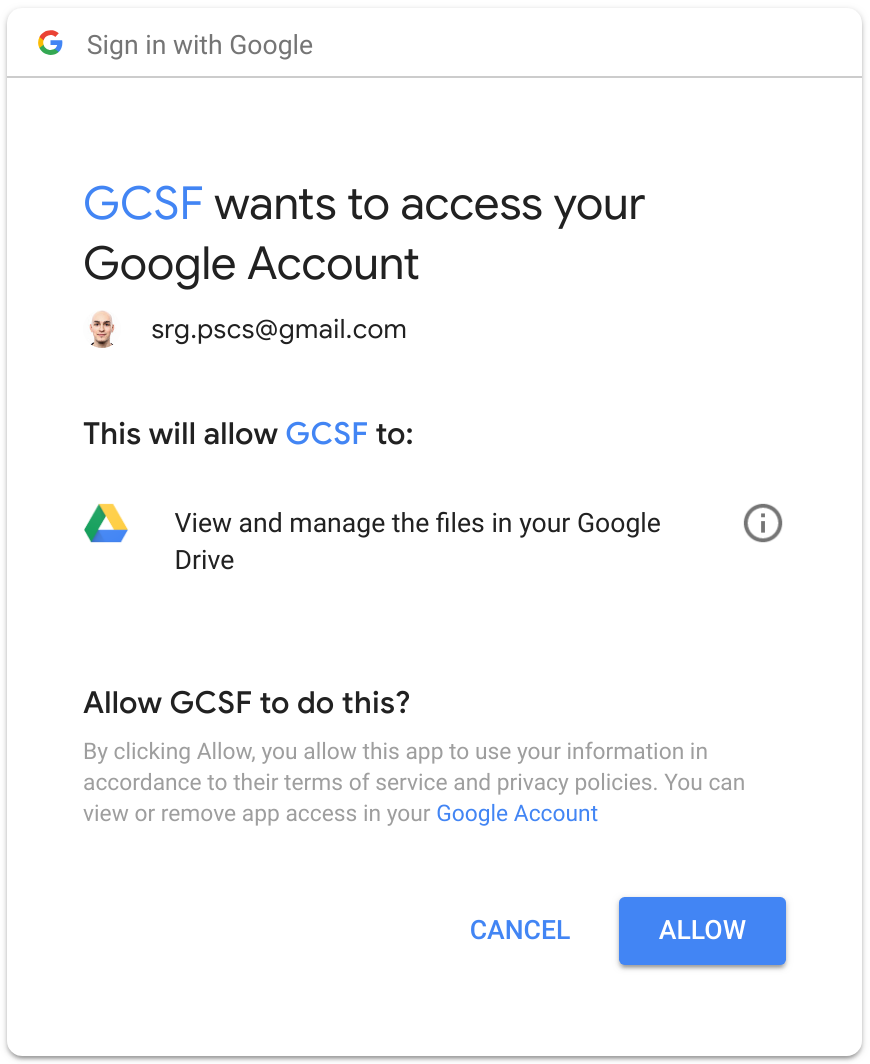
\includegraphics[width=\textwidth]{gcsf_auth}
\end{figure}

\begin{lstlisting}[caption=List of mounted filesystems, frame=single, label=df_output]
$ df -h
Filesystem      Size  Used Avail Use% Mounted on
/dev/nvme0n1p5   64G   45G   17G  74% /
/dev/nvme0n1p6  644G  559G   53G  92% /home
/dev/nvme0n1p1  256M   73M  184M  29% /boot
GCSF             15G   11G  4.6G  70% /mnt/gcsf
\end{lstlisting}

\begin{lstlisting}[caption=Output of mount, frame=single, label=mount_output]
$ mount | grep GCSF
GCSF on /mnt/gcsf type fuse (rw,nosuid,nodev,relatime,user_id=1000,group_id=100,allow_other)
\end{lstlisting}


Now the mount directory can be accessed using a file explorer such as \emph{Ranger} (fig.~\ref{fig:ranger}) or \emph{Thunar} (fig.~\ref{fig:thunar}). Command line programs such as \codeword{ls} work as well (fig.~\ref{fig:ls}). From this point onward, the mount directory can be treated as a regular local directory apart from a few exceptions.

\begin{figure}[tbp]
\caption{Ranger window}
\label{fig:ranger}
\centering
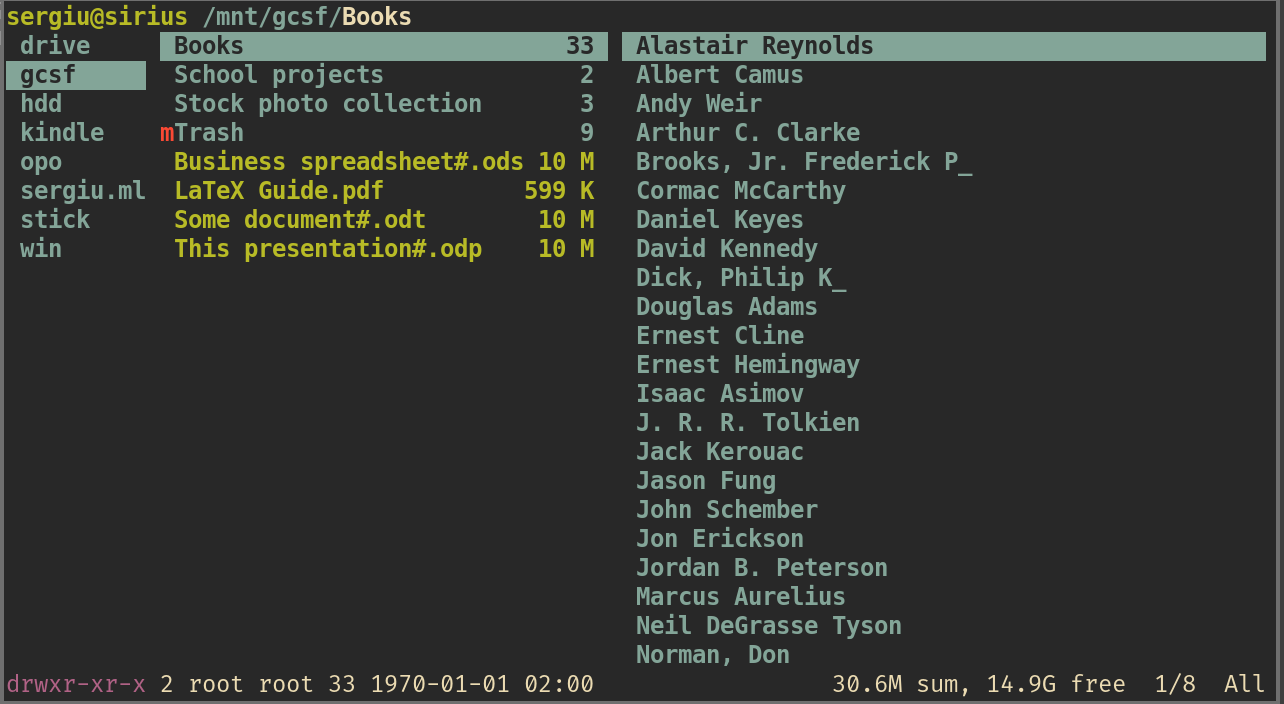
\includegraphics[width=\textwidth]{ranger}
\end{figure}

\begin{figure}[tbp]
\caption{Thunar window}
\label{fig:thunar}
\centering
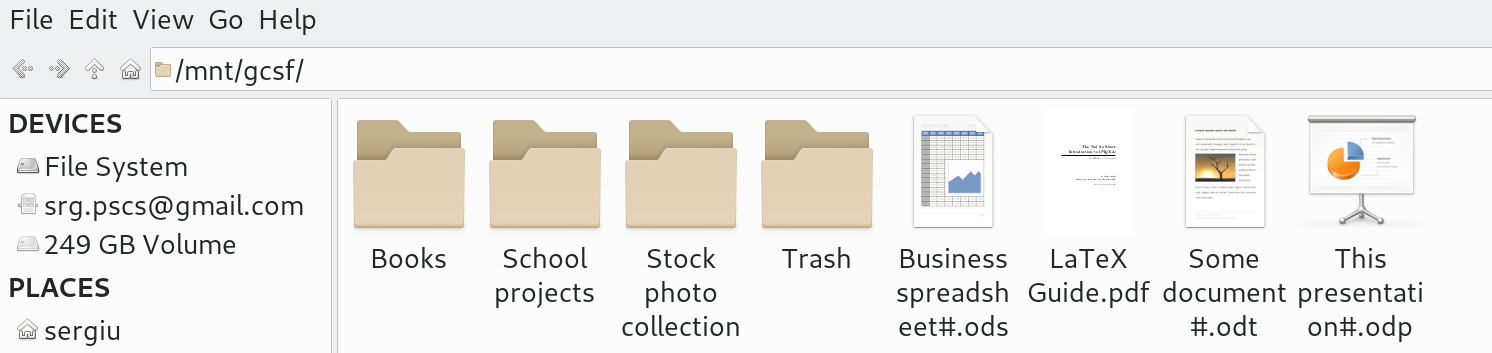
\includegraphics[width=\textwidth]{thunar}
\end{figure}

\begin{figure}[tbp]
\caption{Output of ls}
\label{fig:ls}
\centering
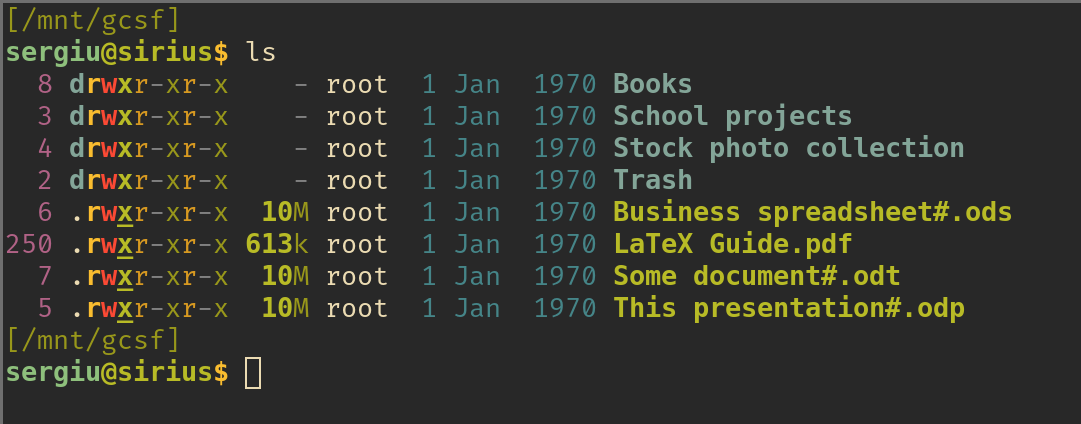
\includegraphics[width=\textwidth]{ls}
\end{figure}

\subsection{Exceptions}

As can be seen in fig.~\ref{fig:ls}, some files have a \codeword{#} symbol attached at the end of their name. This is the case for special Google Drive files, including spreadsheets, docs and slides. Since their file format and size is undefined at this point, GCSF reports the maximum file size supported for these types of files. When such a file is accessed by a user, GCSF chooses the most appropriate filetype and exports the file from Drive. It also adds the appropriate extension to the file name and updates its real size (\ref{gcsf_export}).

\begin{lstlisting}[caption=Exporting Google Drive documents, frame=single, label=gcsf_export]
$ ls "Some document#.odt"
.rwxr-xr-x 10M root  1 Jan  1970 Some document#.odt
$ cp "Some document#.odt" /tmp
$ ls "/tmp/Some document#.odt"
.rwxr-xr-x 8.8k sergiu 12 Jun 18:30 /tmp/Some document#.odt
$ file "/tmp/Some document#.odt"
/tmp/Some document#.odt: OpenDocument Text
\end{lstlisting}




\section{Implementation} \label{implementation}

\subsection{Rust}

Rust is a relatively new systems programming language\footnote{\url{https://www.rust-lang.org/en-US/}} sponsored by the Mozilla Foundation. According to \emph{The Rust Programming Language} book\cite{trpl},

\begin{quote}
Rust is a programming language that helps you write faster, more reliable software. High-level ergonomics and low-level control are often at odds with each other in programming language design; Rust stands to challenge that. Through balancing powerful technical capacity and a great developer experience, Rust gives you the option to control low-level details (such as memory usage) without all the hassle traditionally associated with such control.
\end{quote}

From this description, Rust seems like a good fit for this type of project. However, there are a few specific reasons why I chose it instead of a different language:

\begin{enumerate}
  \item Performance. Rust is in many cases on par with C/C++ in terms of performance. Compared to interpreted languages like Python or Ruby, this is a clear advantage.
  \item Type safety. Any code that may lead to undefined behavior in Rust must be explicitly wrapped within an \codeword{unsafe { }} block, making it the programmer's responsibility to make sure that the code is correct. GCSF does not contain unsafe blocks.
  \item Memory safety.
    \begin{itemize}
      \item \emph{No null pointer dereferences}. Rust does not have the concept of a \codeword{NULL} pointer. Instead, it uses a construct borrowed from the functional world (\codeword{Option<T>}) which encourages the programmer to always check the existence of a packed value.
      \item \emph{No dangling pointers}. Instead of using a garbage collector, Rust has a set of rules that define when and how allocated memory is freed. All of these rules are enforced at compile time, thus eliminating an entire category of runtime errors. The rules are:
      \begin{enumerate}
        \item Any value has a single owner at any given time.
        \item References can not outlive the objects they point to.
        \item At any point, there can be at most one mutable reference \emph{or} any number of immutable (read-only) references to a value.
      \end{enumerate}
      \item \emph{No buffer overruns}
    \end{itemize}
  \item Easy integration of third-party libraries using the \codeword{cargo} package manager and the official package registry\footnote{\url{http://crates.io}}.
  \item Support for the functional paradigm. Rust uses many functional concepts, \emph{closures} and \emph{iterators} being the most popular ones.
  \item Community and growth. According to the \emph{stackoverflow Developer Survey}\footnote{\url{https://insights.stackoverflow.com/survey/2018#most-loved-dreaded-and-wanted}}, developers have chosen Rust as the most loved programming language for three years in a row.
\end{enumerate}

Some of the points stated above are discussed in more depth in Jim Blandy's book \emph{Why Rust?}\cite{why_rust}.

\subsection{FUSE}

FUSE (\textbf{F}ilesystem in \textbf{Use}rspace) is a project that allows users to create virtual filesystems in the user level. Internally, it delegates tasks to a kernel module. As so, users do not have to interact with the kernel directly. FUSE is a popular choice for esoteric filesystems which do not store data themselves. A few notable examples are \emph{sshfs}\footnote{\url{https://github.com/libfuse/sshfs}}, which mounts a remote filesystem using SFTP\footnote{\url{https://tools.ietf.org/html/draft-moonesamy-secsh-filexfer-00}}, and \emph{WikipediaFS}\footnote{\url{http://wikipediafs.sourceforge.net/}} which allows users to view and edit articles locally.

FUSE is made up of two components:
\begin{itemize}
  \item the \textit{fuse} kernel module
  \item the \textit{libfuse} userspace library
\end{itemize}

FUSE filesystems are usually implemented as regular applications that interact with the \textit{libfuse} library. This library provides two interfaces that are useful for defining the behavior of the filesystem. In both cases, the filesystem receives incoming requests from the kernel, which are provided as calls to methods defined in the interface.

First, there is the high-level interface. It uses high-level concepts such as file names and paths in most of its methods. Second, there is the low-level interface. Files are identified using low level concepts such as inodes\cite{tanenbaum}. GCSF uses the latter because of the available language library for Rust.

\subsubsection{High-level interface}

\lstinputlisting[language=C, caption=High-level FUSE interface, frame=single]{fuse.h}

\subsubsection{Low-level interface}
\lstinputlisting[language=C, caption=Low-level FUSE interface, frame=single]{fuse_lowlevel.h}

\subsection{Rust client library}

A Rust implementation of the original FUSE library is available through the \emph{fuse}\footnote{\url{https://crates.io/crates/fuse}} crate. GCSF implements the \codeword{Filesystem} trait defined below.

\lstinputlisting[language=Rust, caption=Rust FUSE interface, frame=single]{fuse.rs}

\subsection{Drive API}

Google provides a REST API for interacting with Drive\footnote{\url{https://developers.google.com/drive/api/v3/about-sdk}}. It also provides official client libraries for multiple programming languages: Java, Javascript, .NET, Objective-C, PHP and Python. There are also early-stage libraries for Dart, Go, Node.js and Ruby.

Unfortunately, Rust is not officially supported. There is however a set of unofficial libraries\footnote{\url{https://github.com/Byron/google-apis-rs}}  programatically generated by Sebastian Thiel\footnote{\url{https://github.com/Byron}}. Although imperfect, they are good enough for the scope of this project.

\subsection{Architecture}

The heart of the application is the \codeword{GCSF} struct. This implements the \codeword{fuse::Filesystem} trait, essentially making it a mountable filesystem. Internally, a \codeword{FileManager} is used for bookkeeping. The \codeword{FileManager} provides all the required functionality for dealing with local files and directories. It keeps track of the file hierarchy, inodes, metadata and performs regular syncs. In order to apply changes remotely on Drive, it uses a \codeword{DriveFacade} linked to the user's account.

These abstractions create a distinct separation of responsibilities. For instance, anything that requires network communication is performed by the \codeword{DriveFacade}. Information about any file can be obtained by simply querying the \codeword{FileManager}. (Un)mounting the file system and responding to system calls is done by \codeword{GCSF}.

\subsection{Caching and laziness}

Because internet connections tend to be slow and imperfect, GCSF aims reduce unnecessary network requests. The main way of achieving this is by caching file contents. Because the content of a given file is unlikely to be modified right after being accessed, it can be stored locally for a small amount of time for faster access. This can be observed by measuring the execution time of successive read operations on the same file (\ref{file_caching}). From a technical standpoint, this feature involves the use of an LRU cache, which is incidentally a remarkably popular programming interview question. Similarly, the reported filesystem capacity and usage values are also cached for a small amount of time.

The second strategy for reducing network requests consists of only uploading new data when necessary. In a UNIX environment, the action of copying a single file might involve a large number of system calls. For instance, the file might have to first be created (using a \codeword{create} call), then have its attributes filled in (using a \codeword{setattr} call), then have its data written (using potentially many \codeword{write} calls with different offsets) and finally be \codeword{flush}ed. Uploading every small change that comes with each individual \codeword{write} call does not make a lot of sense. For this reason, GCSF decides to be lazy and simply store the \codeword{PendingWrite}s in memory. The operations are only performed when a \codeword{flush} call is encountered, and the new file content is uploaded as a whole afterwards.


\begin{lstlisting}[caption=File caching, frame=single, label=file_caching]
$ time file "/mnt/gcsf/LaTeX Guide.pdf"
LaTeX Guide.pdf: PDF document, version 1.5

real    0m2.751s
user    0m0.005s
sys     0m0.005s
$ time file "/mnt/gcsf/LaTeX Guide.pdf"
LaTeX Guide.pdf: PDF document, version 1.5

real    0m0.023s
user    0m0.017s
sys     0m0.001s
\end{lstlisting}


\begin{figure}[bpt]
\caption{GCSF Class Diagram}
\label{fig:gcsf_class_diagram}
\centering
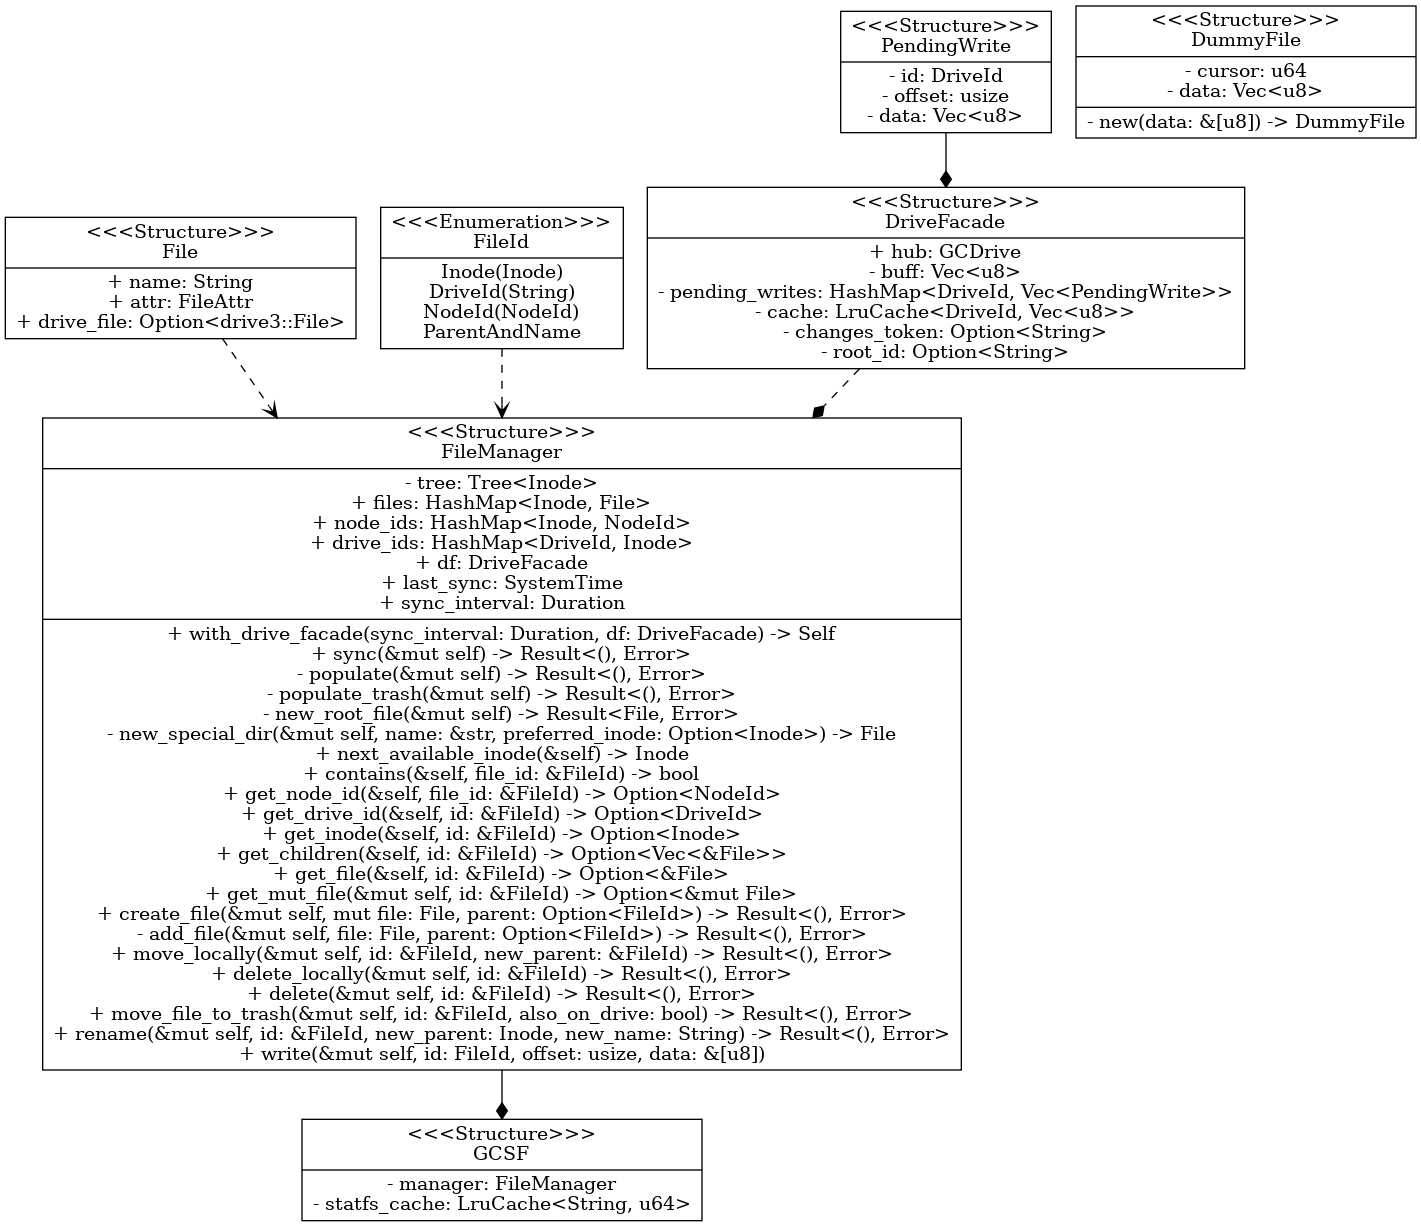
\includegraphics[width=\linewidth]{class_diagram}
\end{figure}


\section{Problems encountered}

As with any sufficiently large project, GCSF involved a series of annoying and obscure problems along the way. I will describe some of the most notable ones in this section.

\subsection{Shared files} \label{shared_files}

The Google Drive REST API provides the \codeword{files.list} endpoint\footnote{\url{https://developers.google.com/drive/api/v3/reference/files/list}} for listing files which meet some criteria. One of the filters that can be applied is the \codeword{sharedWithMe} boolean. It instructs the API to include or ommit files that are shown in the \emph{Shared with me} collection on Drive.

Early implementations of GCSF did not aim to manage shared files at all, as this feature requires extra work to get right. Excluding shared files is easy -- just set \codeword{sharedWithMe = false} in the request. Unfortunately, this does not work, as reported by multiple other developers.\footnote{\url{https://stackoverflow.com/questions/24515151/google-drive-sdk-sharedwithme-false-search-query-not-works}}\footnote{\url{https://github.com/google/google-api-nodejs-client/issues/1136}}\footnote{\url{https://stackoverflow.com/questions/21717592/google-drive-api-files-setq-sharedwithme-false-causes-500-internal-server-error}}. Instead of returning the requested list of files, the API returns a \textbf{500 Internal Server Error}. There is no warning sign for this behavior.

A possible workaround consists of replacing the query with \codeword{`me' in owners}. This is intuitive -- files that are shared with a user are usually not owned by that user, making the two queries partial substitutes for one another. This workaround is not failproof. Exceptions exist and they lead to inconsistent behavior.

The solution I opted for involves a different querying strategy. Instead of asking for all files which are not shared, GCSF asks for files which are direct children of the \emph{My Drive} directory. This is equivalent to setting the query to \codeword{`root' in parents}. Afterwords, the resulting files are processed. In order to explore the rest of the file tree, GCSF recursively queries children of any one of the directories obtained at the previous step. For instance, if the children of the \codeword{root} directory are \codeword{a}, \codeword{b}, \codeword{c}, then the next query will be \codeword{`a' in parents or `b' in parents or `c' in parents}. This essentially explores the file tree one level at a time, resulting in $ O(tree~depth) $ requests.

\subsection{`My Drive' id}

Every file on Google Drive has its own associated string identifier. As discussed in \ref{shared_files}, GCSF populates the local file tree starting with the root (\emph{My Drive}) directory. This is achieved by setting the query \codeword{`root' in parents}, where \codeword{`root'} is a placeholder recognized by the API. However, GCSF needs to know the real identifier for this directory, because files placed in it will use that identifier as their \codeword{parent} field.

The question is: how to obtain this identifier? There is no method for retrieving it from the API.

One way is to get all files that match the \codeword{`root' in parents} query and check the actual identifier that they have in the \codeword{parent} field. GCSF can then use this identifier instead of the \codeword{`root'} placeholder from this point onward. This method usually works, but there were some cases in which the application crashed because of it. For instance, if there are absolutely no files on Drive, the root identifier cannot be obtained. The current implementation works around this limitation by postponing the operation until at least one file is added.

\subsection{File attributes}

The \codeword{fuse} crate represents file attributes using the following struct:

\lstinputlisting[language=Rust, caption=File attributes representation, frame=single]{fileattr.rs}

The \codeword{perm} field is an encoding which describes a file's permissions, essentially stating what any user on the system can and can't do with that file. Any \codeword{Filesytem} can alter these permissions using the \codeword{setattr} method:


\lstinputlisting[language=Rust, caption=Setting file attributes, frame=single]{setattr.rs}

Notice something missing? There is no argument for changing the file permissions. This defeats the entire purpose of recognizing different user permissions and is the reason why GCSF does not enforce this security feature.

\subsection{Updating file metadata on Drive} \label{updating_metadata}

The client library that GCSF uses is generated based on a template which is mostly consistent with the API schema that Google uses. However, there are some inconsistent methods which act as limitations for this project.

One of them regards updates on file metadata. GCSF sometimes has to modify something about a file without modifying its content. For instance, renaming a file or moving it to a different directory are operations which require this sort of behavior. In order to to this, the \codeword{FileUpdateCall} can be used.

For context, most calls exposed by this client library follow the builder pattern\cite{gof}. The general structure is:

\begin{lstlisting}[language=Rust, caption=Setting file attributes, frame=single]
let result = hub.resource().activity(...).doit();
\end{lstlisting}

Or specifically:

\begin{lstlisting}[language=Rust, caption=Setting file attributes, frame=single]
let result = hub.files().copy(...).doit();
let result = hub.files().create(...).doit();
let result = hub.files().list(...).doit();
let result = hub.files().delete(...).doit();
\end{lstlisting}

But the \codeword{update} call is different. Instead of exposing a public \codeword{doit()} method which does all the work, it exposes two alternatives:

\begin{lstlisting}[language=Rust, caption=Setting file attributes, frame=single]
fn upload<RS>(
  self,
  stream: RS,
  mime_type: Mime
) -> Result<(Response, File)>

fn upload_resumable<RS>(
  self,
  resumeable_stream: RS,
  mime_type: Mime
) -> Result<(Response, File)>
\end{lstlisting}

This means that there is no way to update a file's metadata without also providing new content. GCSF works around this by first downloading the current file content and then reuploading it exactly as it is, along with the new metadata. This is extremely wasteful and should be addressed in a future release of the library.

\subsection{Detecting remote changes}

GCSF aims to achieve data consistency in two directions: any change applied locally should also be applied on Drive, and any change applied remotely should also be reflected locally. Remote changes are detected using the \codeword{changes.list} endpoint. GCSF follows the following polling policy:

\begin{itemize}
  \item It should ask for remote changes and apply them locally right before serving user requests.
  \item It should not do this everytime. There should be a user-defined cooldown period between syncs.
\end{itemize}

This generally works. Files added/removed/modified on the web or mobile client are picked up by GCSF after a short while. No wasteful network traffic is generated, as would be the case with regular polling. The delay perceived by the user is present but not significant as it only occurs every once in a while.

But there is a problem. The API seems to make up its own mind and only return the requested changes when it wants. Sometimes, this happens almost instantly. On other occasions, the user has to manually intervene and remount the filesystem in order to preserve its consistency. This can lead to problems which impair user experience.

\subsection{Moving files to trash}

A problem similar to \ref{updating_metadata} occurs when attempting to move a file to trash. From a technical standpoint, this can be done by querying the \codeword{files.update} endpoint and setting \codeword{trashed=true} in the request. However, this results in an internal server error which states that the \codeword{trashed} field cannot be set manually. There seems to be no straightforward alternative, so at the moment all file deletions performed by GCSF are permanent.

% Data used in charts

\pgfplotstableread[row sep=\\,col sep=&]{
fileSize & gcsf & google-drive-ocamlfuse & gdrivefs \\
1 MB     & 1.3  & 1.5 & 0.7 \\
10 MB    & 2.3  & 1.8 & 6.9 \\
50 MB    & 4.9  & 5.4 & 26  \\
100 MB   & 6.8  & 8.2 & 60  \\
200 MB   & 8.2  & 9.9 & 107 \\
}\freshreaddata

\pgfplotstableread[row sep=\\,col sep=&]{
fileSize & gcsf & google-drive-ocamlfuse & gdrivefs \\
1 MB     & 0.0  & 0.0                    & 0.5   \\
10 MB    & 0.0  & 0.2                    & 4.5   \\
50 MB    & 0.1  & 0.7                    & 27    \\
100 MB   & 0.3  & 1.4                    & 50    \\
200 MB   & 0.5  & 2.8                    & 95    \\
}\cachereaddata

\pgfplotstableread[row sep=\\,col sep=&]{
Mount & gcsf & google-drive-ocamlfuse & gdrivefs \\
      & 8.17 & 0.78                   & 0.02     \\
}\mountingtimes

\pgfplotstableread[row sep=\\,col sep=&]{
Tree & gcsf & google-drive-ocamlfuse & gdrivefs \\
     & 0.26 & 2.35                   & 62.79    \\
}\treetimes

% EOData


\chapter{Performance evaluation}\label{performance_evaluation}

Although comparing GCSF with similar tools is a fuzzy task, I will attempt to construct an appropriate performance analysis. For this purpose I have selected two other projects:

\begin{itemize}
  \itemsep0em
  \item \emph{dsoprea/GDriveFS}~\cite{dsoprea/GDriveFS}, which I personally used prior to starting work on GCSF.
  \item \emph{astrada/google-drive-ocamlfuse}~\cite{astrada/google-drive-ocamlfuse} -- the most popular project of those mentioned in this section.
\end{itemize}

Besides the two, there are many other similar projects. Most of them are either in early stages of development, abandoned, or serve a different purpose:

\begin{itemize}
  \itemsep0em
  \item \emph{thejinx0r/node-gdrive-fuse}~\cite{thejinx0r/node-gdrive-fuse} -- unmaintained since February 2016.
  \item \emph{joe42/CloudFusion}~\cite{joe42/CloudFusion} -- unmaintained since January 2015.
  \item \emph{S2Games/drivefs}~\cite{S2Games/drivefs} -- unmaintained since June 2014.
  \item \emph{BYVoid/gdrive}~\cite{BYVoid/gdrive} -- unmaintained since October 2013.
  \item \emph{jcline/fuse-google-drive}~\cite{jcline/fuse-google-drive} -- unmaintained since September 2012.
  \item \emph{thejinx0r/DriveFS}~\cite{thejinx0r/DriveFS} -- undocumented as of June 2018 and still in early stages of development.
  \item \emph{zond/futon}~\cite{zond/futon} -- unmaintained since December 2014. In addition, it is \emph{``right now, and probably forever, read only''} according to the documentation.
  \item \emph{dweidenfeld/plexdrive}~\cite{dweidenfeld/plexdrive} -- only allows read-only access and targets media streaming.
\end{itemize}

As such, I have decided to exclude these projects from my analysis and benchmarks. Here is a brief comparison of the chosen projects, as of 23 June 2018:

\vspace{1em}

\makebox[.9\textwidth]{
\begin{tabular}{cc|c|c|c|c|l}
\cline{3-5}
& & \multicolumn{1}{ c| }{GCSF} & \multicolumn{1}{ c|}{GDriveFS} & \multicolumn{1}{ c| }{google-drive-ocamlfuse} \\ \cline{1-5}

\multicolumn{1}{ |l| }{\multirow{7}{*}{\shortstack[l]{Github \\ Statistics}}} &
\multicolumn{1}{  l| }{Owner}        & Sergiu Pușcaș & Dustin Oprea & Alessandro Strada \\ \cline{2-5}
\multicolumn{1}{ |l| }{}             &
\multicolumn{1}{  l| }{First Commit} & April 2018    & August 2012  & May 2012          \\ \cline{2-5}
\multicolumn{1}{ |l| }{}             &
\multicolumn{1}{  l| }{Commits}      & 130           & 395          & 511               \\ \cline{2-5}
\multicolumn{1}{ |l| }{}             &
\multicolumn{1}{  l| }{Releases}     & 1             & 23           & 71                \\ \cline{2-5}
\multicolumn{1}{ |l| }{}             &
\multicolumn{1}{  l| }{Contributors} & 1             & 6            & 12                \\ \cline{2-5}
\multicolumn{1}{ |l| }{}             &
\multicolumn{1}{  l| }{Stars}        & 11            & 491          & 2086              \\ \cline{2-5}
\multicolumn{1}{ |l| }{}             &
\multicolumn{1}{  l| }{Forks}        & 0             & 81           & 153               \\ \cline{1-5}

\multicolumn{1}{ |l| }{\multirow{2}{*}{\shortstack[l]{Technical \\ Details}}} &
\multicolumn{1}{  l| }{Language}     & Rust          & Python 2.7   & OCaml             \\ \cline{2-5}
\multicolumn{1}{ |l| }{}             &
\multicolumn{1}{  l| }{LoC}          & 2093          & 5232         & 7962              \\ \cline{1-5}
\end{tabular}
}

\vspace{1em}

In the next sections I will discuss each of these projects from a technical standpoint and from a user perspective.

\section{GDriveFS}

As of June 2018, \emph{GDriveFS} aims to be \emph{``an innovative FUSE wrapper for Google Drive''}~\cite{dsoprea/GDriveFS}. It has been in development for the past six years, accumulating along the way a total of almost 400 commits, 23 releases, 6 contributors and 81 forks. As a consequence, GDriveFS has more features than GCSF and its longevity makes it a time-proven piece of software. This has been consistent with my personal experience. GDriveFS worked out of the box in most situations where I attempted to use it.

Unfortunately, I also encountered some issues. I will walk through a first time setup of this application in order to illustrate its drawbacks. First, we create a new virtual environment using \codeword{virtualenv} in order to avoid conflicts between global Python packages and the local requirements of GDriveFS. We can easily install GDriveFS in this environment as a \codeword{pip} package.

\begin{lstlisting}[basicstyle=\footnotesize\ttfamily,frame=single,caption=Creating a virtual environment and installing GDriveFS]
$ virtualenv2 gdrivefs
New python executable in ./gdrivefs/bin/python2
Also creating executable in ./gdrivefs/bin/python
Installing setuptools, pip, wheel...done.
$ source gdrivefs/bin/activate
(gdrivefs) $ pip install gdrivefs
Collecting gdrivefs
Collecting fusepy==2.0.2 (from gdrivefs)
Collecting httplib2==0.8 (from gdrivefs)
[...]
Successfully installed gdrivefs-0.14.9 [...]
\end{lstlisting}

Now we are ready to run into our first problem. The official documentation suggests using \codeword{gdfstool auth_automatic} in order to log in with our Google account~\cite{GDriveFS_README}. However, we encounter an error:

\begin{lstlisting}[basicstyle=\footnotesize\ttfamily,frame=single,caption=GDriveFS nonexistent authentication command]
(gdrivefs) $ gdfstool auth_automatic
usage: gdfstool [-h] {auth,mount} ...
gdfstool: error: argument command: invalid choice: `auth_automatic' (choose from `auth', `mount')
\end{lstlisting}

It seems that there is an inconsistency between the documentation and the application itself. No problem. We can follow the suggestion provided by the error message and execute \codeword{gdfstool auth} instead. We provide the \codeword{-o} flag in order to open the authentication form in a browser window. After logging in and allowing the application to access our account, we are ready to feed the access code into \codeword{gdfstool}:

\begin{lstlisting}[frame=single,caption=GDriveFS authentication error]
(gdrivefs) $ gdfstool auth -a /tmp/credentials "$AUTH_CODE"
[...]
gdrivefs.errors.AuthorizationFailureError: Could not do auth-exchange (this was either a legitimate error, or the auth-exchange was attempted when not necessary): [SSL: CERTIFICATE_VERIFY_FAILED] certificate verify failed (_ssl.c:726)
\end{lstlisting}

This is strange. After researching the problem, we find a relevant open issue on this subject~\cite{gdrivefs_ssl_handshake_error}. According to user \emph{blitz313}, the root cause is one of the dependencies. Manual installation of package \codeword{httplib2-0.10.3} (instead of the required version \codeword{0.8}) seems to solve this problem and we can finally mount the filesystem:

\begin{lstlisting}[frame=single,caption=GDriveFS filesystem mount]
(gdrivefs) $ gdfstool mount /tmp/credentials /mnt/gdrivefs
(gdrivefs) $ ls /mnt/gdrivefs/
drwxrwxrwx@    - sergiu 11 Jun 18:56 Books
drwxrwxrwx@    - sergiu 11 Jun 19:04 School projects
drwxrwxrwx@    - sergiu 11 Jun 18:59 Stock photo collection
.rw-rw-rw-@ 1.0k sergiu 11 Jun 18:57 Business spreadsheet#
.rw-rw-rw-@ 613k sergiu 11 Jun 19:38 LaTeX Guide.pdf
.rw-rw-rw-@ 1.0k sergiu 12 Jun 15:27 Some document#
.rw-rw-rw-@ 1.0k sergiu 11 Jun 18:57 This presentation#
\end{lstlisting}

From this point on, most operations perform as expected. My biggest issue with GDriveFS is its async I/O strategy. Files written to the file system are not instantly updated locally or on Drive. Reading a file too soon after writing to it can cause data inconsistency. In my benchmarks, writing files larger than \mbox{10 MB} and reading them immediatelly afterwards often resulted in checksum failures. Reading the same file multiple times in a row can also result in different outputs.

In the situations where GDriveFS did work, it required significantly more time than its competitors. This may be attributed to the fact that it is implemented in Python, which is known to be slower than statically-typed compiled languages.

Overall, the experience can only be described as messy. GDriveFS makes it difficult to reason about the state of the operations performed, and what you see is not always what you get.

\section{google-drive-ocamlfuse}

Compared to GDriveFS, google-drive-ocamlfuse is the result of the collective effort of twice as many contributors. As of June 2018, it has been starred by more than 2000 users on GitHub. For comparison, the programming language it is written in only has 1850 stars~\cite{ocaml}.

This project is implemented in OCaml~\cite{ocaml-website}, ``an industrial strength programming language supporting functional, imperative and object-oriented styles''. According to open-source software developer Thomas Leonard, OCaml can often achieve better performance compared to Python~\cite{python_to_ocaml_retrospective}. Whether or not this is the case in general, it is certainly reflected in the case of this project. As it turns out, it is the best performer in several categories described in section~\ref{benchmarks}.

From a user perspective, google-drive-ocamlfuse also has its flaws. For once, it does not support authentication using a generated code. This makes it more difficult to use on a headless machine, but it is not a problem for most users. Installation can also be tricky. I have personally run into issues such as~\cite{opam-depext-issue} while trying to set up the file system. The Arch Linux package~\cite{google-drive-ocamlfuse-aur} does not automatically pull in all dependencies, requiring manual installation of several packages.

However, after setting the file system up, all of these issues disappear. The user experience is unimpaired. In all tests, there were no cases of data inconsistency or file system errors.

\section{Benchmarks} \label{benchmarks}

\subsection{Methodology}

All tests were performed on a machine with the following specifications:

\begin{itemize}
  \setlength\itemsep{-0.4em}
  \item Intel(R) Xeon(R) CPU E5-2650 v4 @ 2.20GHz
  \item SSD storage
  \item 4 GB RAM
  \item 3 Gb/s internet connection
\end{itemize}

Unless stated otherwise, all file systems were mounted using their default configuration. All results reported in the following sections are averaged among 10 successive executions. The test account has been artificially populated with 2000 files and 100 directories, totalling 2.8 GB. The maximum depth of any file in the the file tree is 4.

\subsection{Mounting and startup}

Compared to google-drive-ocamlfuse and GDriveFS, GCSF populates the file tree at mount time. As discussed in \ref{shared_files}, the startup time of GCSF grows linearly with the depth of the file tree. This means that the file system will take longer to load deeply nested directories, but it has no problems with a large number of files in a shallow file tree.

As seen in fig.~\ref{fig:mount_benchmark}, constructing the file tree at mount time increases the loading time of the file system, but it significantly improves subsequent operations. More on this in section \ref{list_benchmark}.


\begin{figure}[bpt]
\centering
\begin{tikzpicture}
    \begin{axis}[
            ybar,
            bar width=2cm,
            width=.9\textwidth,
            height=.4\textwidth,
            legend style={at={(0.5,1)},
                anchor=north,legend columns=-1},
            symbolic x coords={},
            xtick=data,
            nodes near coords,
            nodes near coords align={vertical},
            ymin=0,ymax=12,
            ylabel={Time (seconds)},
            every node near coord/.append style={/pgf/number format/.cd, fixed,1000 sep={}}
        ]
        \addplot+[rustcolor,draw=black] table[x=Mount,y=gcsf]{\mountingtimes};
        \addplot+[ocamlcolor,draw=black] table[x=Mount,y=google-drive-ocamlfuse]{\mountingtimes};
        \addplot+[pythoncolor,draw=black] table[x=Mount,y=gdrivefs]{\mountingtimes};
        \legend{GCSF, google-drive-ocamlfuse, GDriveFS}
    \end{axis}
\end{tikzpicture}
\caption{Mounting a file system with 2000 files and 100 directories, nested on 4 levels.}
\label{fig:mount_benchmark}
\end{figure}


\subsection{File listing} \label{list_benchmark}

One of the first operations performed after mounting the file system is in many cases a file listing. Whether this is achieved using a command line tool such as \codeword{ls} or a GUI file explorer, the file system has to respond to the same system calls -- mainly \codeword{readdir} and \codeword{lookup}. For this benchmark, I decided to measure the execution time of the \codeword{tree} command \cite{tree_man_page}. This  command explores an entire directory recursively, constructing an ASCII tree-like structure of all files and directories.

This is where the longer mount time of GCSF pays off. As seen in fig.~\ref{fig:tree_benchmark}, GCSF is one order of magnitude faster than google-drive-ocamlfuse, and two orders of magnitude faster than GDriveFS. It should be noted that the first listing performed on google-drive-ocamlfuse is considerably slower than subsequent listings -- approximately 60 seconds -- because of the empty cache. This outlier is not included in the computed average.


\begin{figure}[bpt]
\centering
\begin{tikzpicture}
    \begin{axis}[
            ybar,
            bar width=2cm,
            width=.9\textwidth,
            height=.4\textwidth,
            legend style={at={(0.5,1)},
                anchor=north,legend columns=-1},
            symbolic x coords={},
            xtick=data,
            nodes near coords,
            nodes near coords align={vertical},
            ymin=0,ymax=92,
            ylabel={Time (seconds)},
            every node near coord/.append style={/pgf/number format/.cd, fixed,1000 sep={}}
        ]
        \addplot+[rustcolor,draw=black] table[x=Tree,y=gcsf]{\treetimes};
        \addplot+[ocamlcolor,draw=black] table[x=Tree,y=google-drive-ocamlfuse]{\treetimes};
        \addplot+[pythoncolor,draw=black] table[x=Tree,y=gdrivefs]{\treetimes};
        \legend{GCSF, google-drive-ocamlfuse, GDriveFS}
    \end{axis}
\end{tikzpicture}
\caption{Listing all files and directories recursively.}
\label{fig:tree_benchmark}
\end{figure}


\subsection{Reading -- empty cache} \label{reading_empty_cache}

The target of this test is to measure the execution time required for computing an MD5 checksum of a randomly generated file. This allows us to check whether or not the file content is retrieved by each file system in its entirety and without errors. Although computing the checksum takes some time in itself, it only affects the measured times marginally.


\begin{figure}[bpt]
\centering
\begin{tikzpicture}
    \begin{axis}[
            ybar,
            bar width=.5cm,
            width=.95\textwidth,
            height=.5\textwidth,
            legend style={at={(0.5,1)},
                anchor=north,legend columns=-1},
            symbolic x coords={1 MB,10 MB,50 MB,100 MB,200 MB},
            xtick=data,
            nodes near coords,
            nodes near coords align={vertical},
            ymin=0,ymax=120,
            ylabel={Time (seconds)},
            every node near coord/.append style={/pgf/number format/.cd, fixed,1000 sep={}}
        ]
        \addplot+[rustcolor,draw=black] table[x=fileSize,y=gcsf]{\freshreaddata};
        \addplot+[ocamlcolor,draw=black] table[x=fileSize,y=google-drive-ocamlfuse]{\freshreaddata};
        \addplot+[pythoncolor,draw=black] table[x=fileSize,y=gdrivefs]{\freshreaddata};
        \legend{GCSF, google-drive-ocamlfuse, GDriveFS}
    \end{axis}
\end{tikzpicture}
\caption{Reading a file when the cache is empty.}
\label{fig:fresh_read_benchmark}
\end{figure}

As seen in fig.~\ref{fig:fresh_read_benchmark}, google-drive-ocamlfuse tends to perform best on small files. GCSF is slower because it makes an additional request to Google Drive: first it creates an empty file and then it updates the file content. However, the performance changes for larger files. In this case, an additional network request becomes insignificant compared to each file system's efficiency of processing operations internally. As it turns out, GCSF performs slightly better than google-drive-ocamlfuse.

Not the same can be said about GDriveFS. Its execution time grows almost linearly with the file size. Moreover, the computed checksums are incorrect in many cases. Waiting for the file system to resynchronize with Drive may fix these errors, but the inconvenience of not knowing whether or not the file system introduced errors to user data still exists.

\begin{table}[h]
\makebox[\textwidth]{
\begin{tabular}{|l|l|l|}
\hline
\multirow{2}{*}{File size (MB)} & \multicolumn{2}{l|}{Checksum errors (\%)} \\ \cline{2-3}
                                & Fresh read          & Cached read         \\ \hline
1                               & 20                  & 10                  \\ \hline
10                              & 40                  & 60                  \\ \hline
50                              & 90                  & 70                  \\ \hline
100                             & 80                  & 100                 \\ \hline
200                             & 90                  & 100                 \\ \hline
\end{tabular}
}
\caption{Checksum errors reported when reading from GDriveFS} \label{tab:checksum_errors}
\end{table}

\subsection{Reading -- cached}

Both GCSF and google-drive-ocamlfuse provide a caching mechanism. GCSF uses an in-memory least recently used (LRU) cache in order to preserve file content for some time after retrieving it from Drive, whereas google-drive-ocamlfuse uses an on-disk SQLite 3 database. Both methods have their advantages and disadvantages. Retrieving data from memory is faster but the available capacity can be a limiting factor. Caching on disk removes this limitation, at the cost of slower speeds.

As far as I can tell, GDriveFS only caches authentication tokens and the structure of the file tree. This is reflected in fig.~\ref{fig:cached_read_benchmark}. As was the case in section \ref{reading_empty_cache}, checksum errors still occur with GDriveFS. The exact values can be found in table \ref{tab:checksum_errors}.

\begin{figure}[bpt]
\centering
\begin{tikzpicture}
    \begin{axis}[
            ybar,
            bar width=.6cm,
            width=\textwidth,
            height=.5\textwidth,
            legend style={at={(0.5,1)},
                anchor=north,legend columns=-1},
            symbolic x coords={1 MB,10 MB,50 MB,100 MB,200 MB},
            xtick=data,
            nodes near coords,
            nodes near coords align={vertical},
            ymin=0,ymax=110,
            ylabel={Time (seconds)},
        ]
        \addplot+[rustcolor,draw=black] table[x=fileSize,y=gcsf]{\cachereaddata};
        \addplot+[ocamlcolor,draw=black] table[x=fileSize,y=google-drive-ocamlfuse]{\cachereaddata};
        \addplot+[pythoncolor,draw=black] table[x=fileSize,y=gdrivefs]{\cachereaddata};
        \legend{GCSF, google-drive-ocamlfuse, GDriveFS}
    \end{axis}
\end{tikzpicture}
\caption{Reading a cached file.}
\label{fig:cached_read_benchmark}
\end{figure}


\chapter{Conclusion}
Some conclusion here.


\begin{appendices}
\chapter{Rust FUSE library} \label{appendix:rust_fuse}
\lstinputlisting[language=Rust, caption=Rust FUSE interface, frame=single]{fuse.rs}
\end{appendices}

% \Urlmuskip=0mu plus 1mu\relax
\bibliographystyle{plain}
\raggedright
\bibliography{bibliography}

\end{document}
